% Beamer version of the standalone 22-slide deck.
% Compile:  xelatex talk.tex   (run twice for refs)
\documentclass[aspectratio=169,11pt]{beamer}
\usepackage{fontspec}
\setsansfont{Helvetica Neue}[Scale=0.95]
\setmonofont{Menlo}[Scale=0.78]
\usepackage{xcolor}
\usepackage{graphicx}
\usepackage{tcolorbox}
\tcbuselibrary{skins,breakable}
\usepackage{tikz}
\usepackage{array}

% --- palette (matches the Marp standalone deck) ---
\definecolor{titlenavy}{HTML}{1A3A6A}
\definecolor{l1grey}{HTML}{7F7F7F}
\definecolor{l2amber}{HTML}{FFBB78}
\definecolor{l2dark}{HTML}{D97706}      % readable bold L2 on white
\definecolor{l3orange}{HTML}{FF7F0E}
\definecolor{taskblue}{HTML}{1F77B4}
\definecolor{bggreen}{HTML}{2CA02C}
\definecolor{dontred}{HTML}{D62728}
\definecolor{cardbg}{HTML}{FAFAFA}
\definecolor{codebg}{HTML}{F4F4F4}

\usetheme{default}
\setbeamertemplate{navigation symbols}{}
\setbeamercolor{frametitle}{fg=titlenavy,bg=white}
\setbeamercolor{normal text}{fg=black,bg=white}
\setbeamerfont{frametitle}{size=\Large,series=\bfseries}
\setbeamertemplate{itemize item}{\color{titlenavy}\textbullet}
\setbeamertemplate{itemize subitem}{\color{titlenavy}\textendash}
\setbeamertemplate{footline}{%
  \hfill\raisebox{6pt}{\tiny\color{gray}\insertframenumber\hspace{6mm}}%
}
\setbeamertemplate{frametitle}{%
  \vspace{6pt}\hspace{4pt}\insertframetitle\par\vspace{-2pt}%
}

% --- macros ---
\newcommand{\bignum}[3]{%
  \centering
  {\fontsize{40pt}{44pt}\selectfont\textbf{\textcolor{#1}{#2}}}\par
  \vspace{4pt}{\small\textbf{\textcolor{#1}{#3}}}\par
}

\newcommand{\personacard}[4]{%
  \begin{tcolorbox}[
    colback=cardbg, colframe=#1, boxrule=1.2pt, arc=3pt,
    left=6pt, right=6pt, top=4pt, bottom=4pt,
    valign=top, height=4.6cm,
  ]
    \textbf{\textcolor{#1}{#2}}\\[2pt]
    \small #3\\[6pt]
    \scriptsize\textcolor{gray!50!black}{#4}
  \end{tcolorbox}%
}

\newcommand{\patternbox}[3]{%
  \begin{tcolorbox}[
    colback=cardbg, colframe=#1, boxrule=1.2pt, arc=3pt,
    left=8pt, right=8pt, top=3pt, bottom=3pt,
  ]
    {\textbf{\textcolor{#1}{#2}}}\par
    \small #3
  \end{tcolorbox}%
}

\newcommand{\codeblock}[1]{%
  \begin{tcolorbox}[colback=codebg, colframe=codebg, arc=3pt, left=8pt, right=8pt, top=4pt, bottom=4pt]
    \ttfamily\footnotesize #1
  \end{tcolorbox}%
}

\begin{document}

% ===== Slide 0 — Title =====
{\setbeamertemplate{footline}{}
\begin{frame}[plain]
  \vfill
  \begin{center}
    {\fontsize{36pt}{40pt}\selectfont\bfseries\textcolor{titlenavy}{Prompt engineering, in practice}}\par
    \vspace{10pt}
    {\Large\textcolor{gray!50!black}{Three users, one forecasting task,\\a factor-of-three in error}}
  \end{center}
  \vfill
  \begin{center}\small\textcolor{gray}{JRC C4 \quad{\textperiodcentered}\quad Dermot O'Brien \quad{\textperiodcentered}\quad 2026}\end{center}
\end{frame}}

% ===== Slide 1 — Headline =====
\begin{frame}{The headline}
  \vspace{18pt}
  \begin{columns}[t,onlytextwidth]
    \begin{column}{0.32\textwidth}\bignum{l1grey}{10.76\%}{L1 --- beginner}\end{column}
    \begin{column}{0.32\textwidth}\bignum{l2dark}{5.52\%}{L2 --- average}\end{column}
    \begin{column}{0.32\textwidth}\bignum{l3orange}{3.43\%}{L3 --- pro}\end{column}
  \end{columns}
  \vfill
  \begin{center}\small\color{gray!40!black}
    MAPE on a held-out 168-hour forecast of German hourly electricity load.\\
    Same data. Same target. Same AI agent (Claude Code, Opus 4.7).
  \end{center}
  \vspace{12pt}
\end{frame}

% ===== Slide 2 — Puzzle =====
\begin{frame}
  \vspace{1.2cm}
  \begin{center}
    {\fontsize{30pt}{34pt}\selectfont\bfseries What changed between these three runs?}
  \end{center}
  \vfill
  \begin{center}\large\color{gray!40!black}
    Three things: the prompt itself \quad\textperiodcentered\quad the project workspace
    \quad\textperiodcentered\quad what we asked for as output.
  \end{center}
  \vspace{1cm}
\end{frame}

% ===== Slide 3 — The task =====
\begin{frame}{The task}
  \begin{itemize}
    \item Forecast \textbf{168 hours} (one week) of hourly German electricity load
    \item Test window: \textbf{2020-01-01 to 2020-01-07} (held out)
    \item Training data: 2015-01-01 onward, hourly, $\sim$50{,}000 rows
    \item Source: \textbf{Open Power System Data} / ENTSO-E
    \item Univariate: load series + features derivable from the timestamp
  \end{itemize}
\end{frame}

% ===== Slide 4 — The data =====
\begin{frame}{The data}
  \begin{center}
    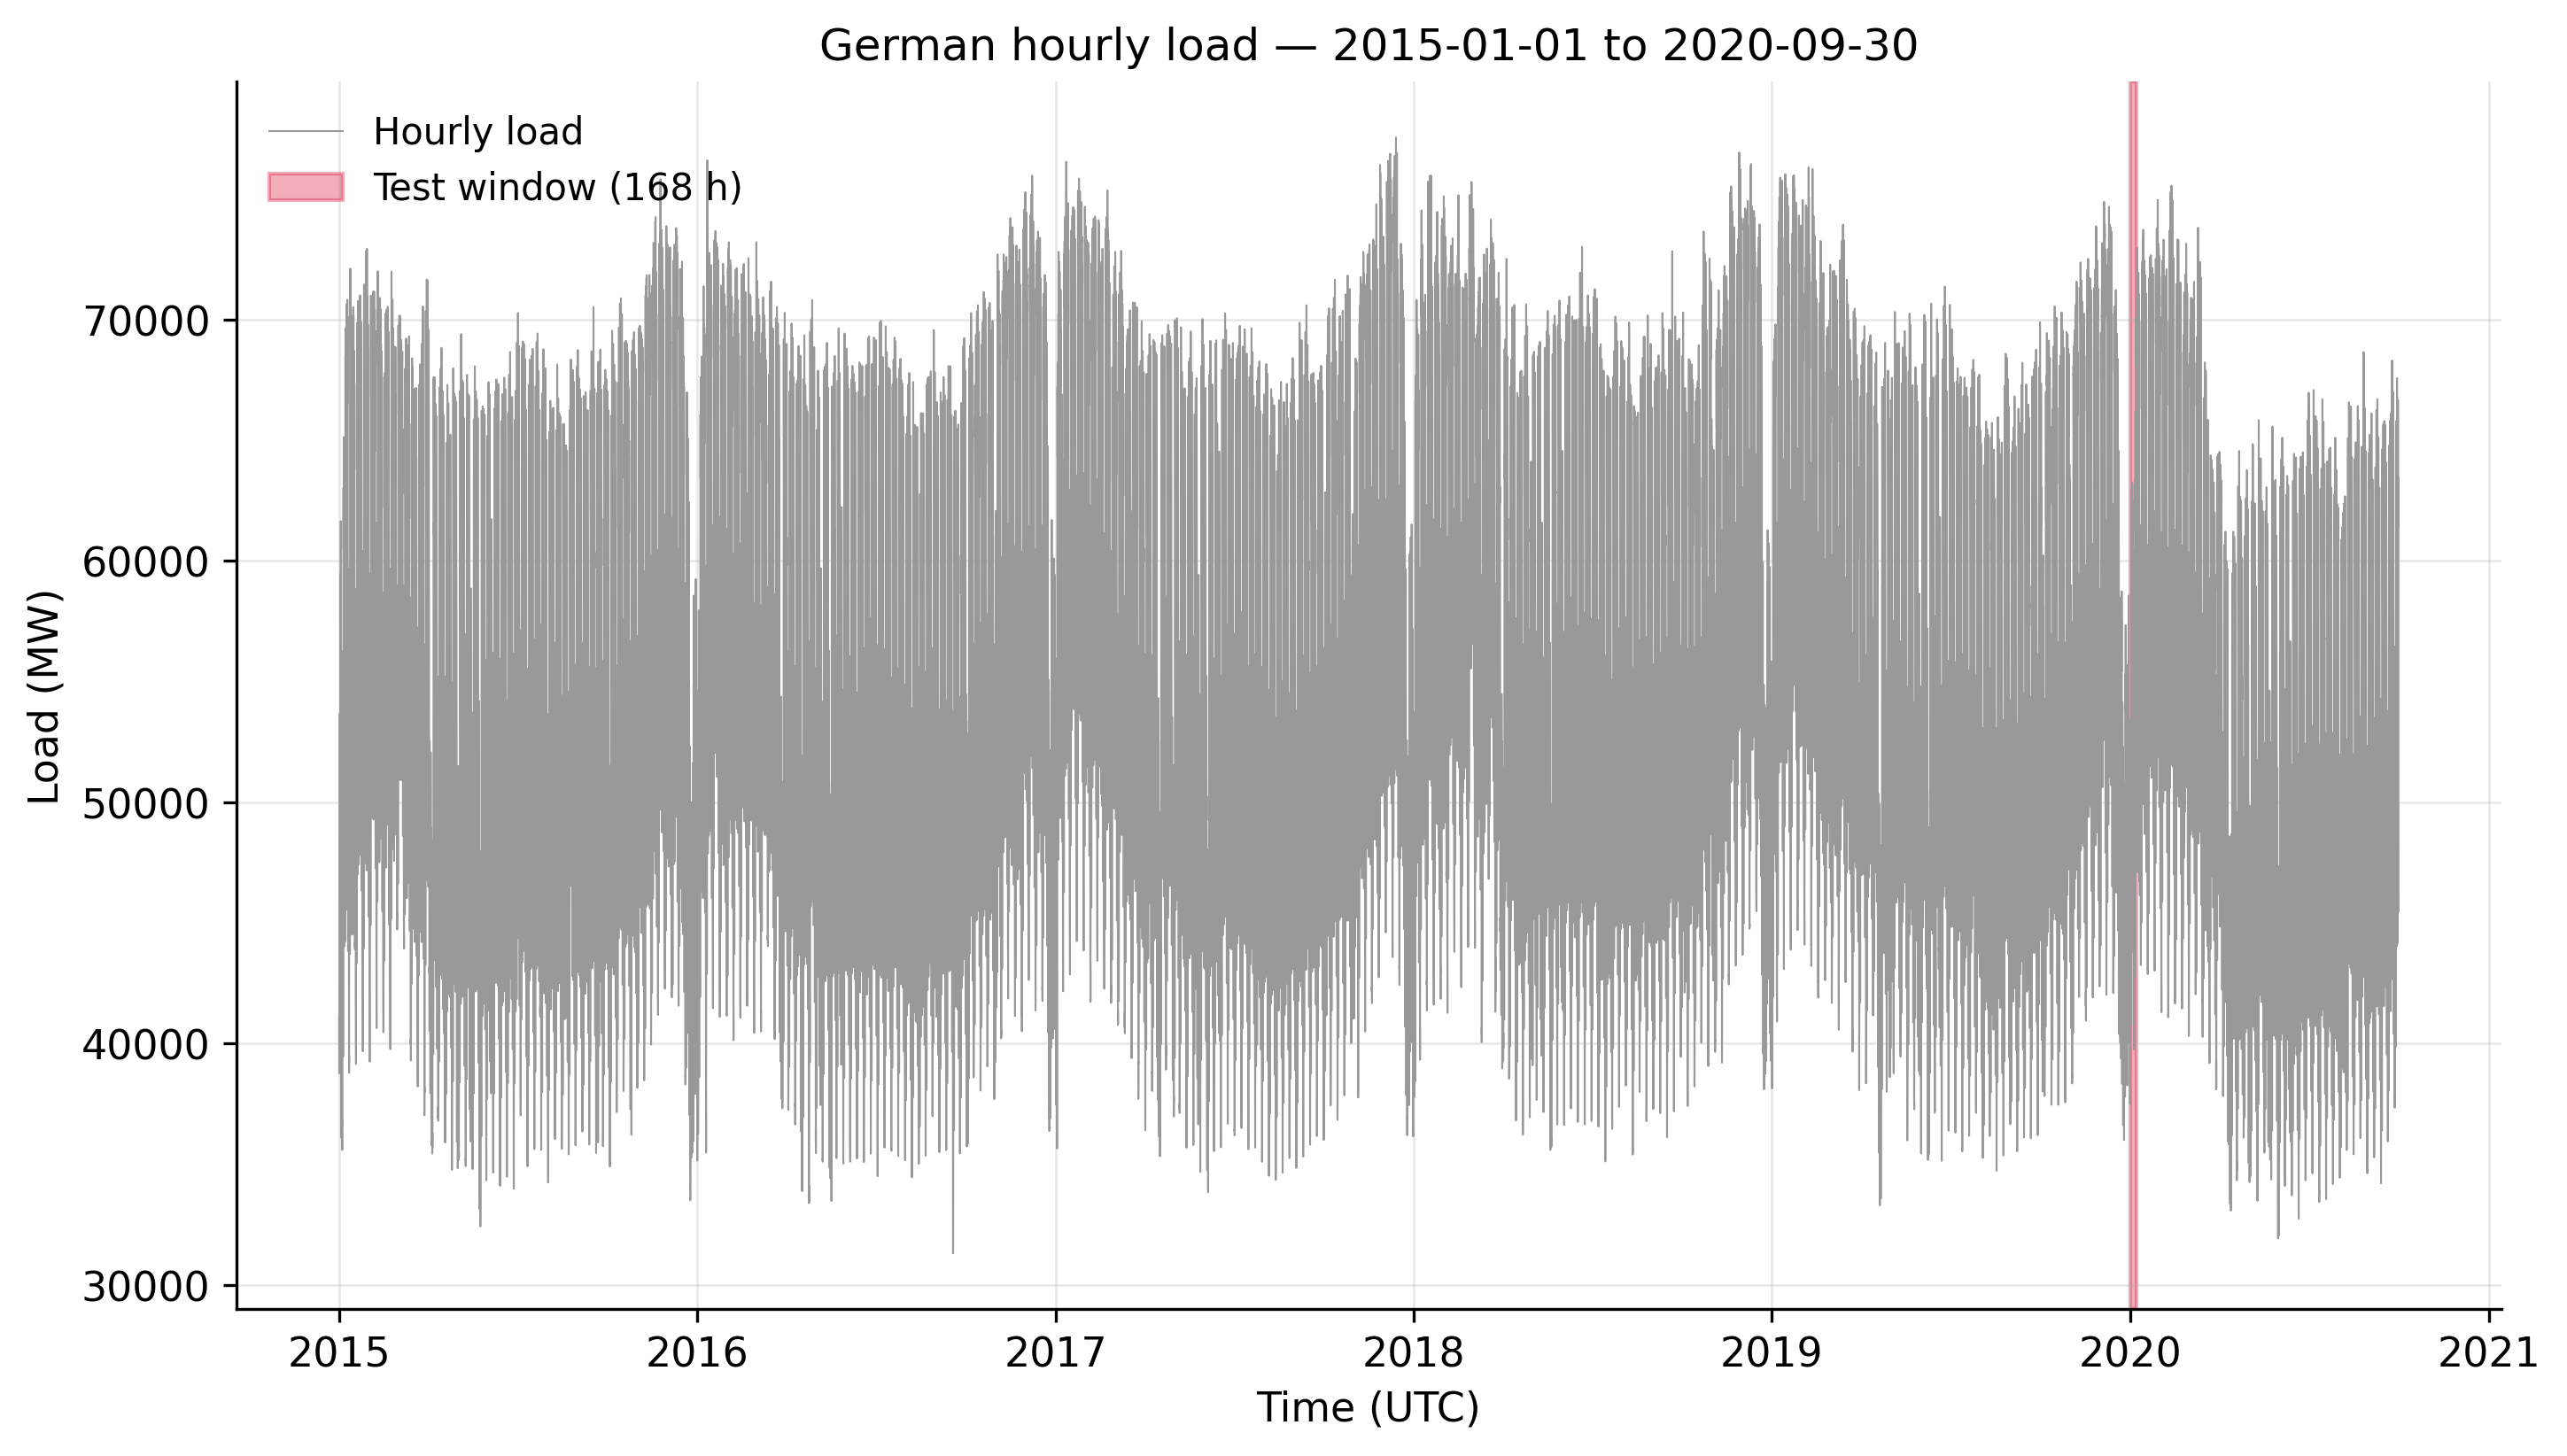
\includegraphics[height=0.78\textheight]{../runs/L3/figures/01_overview.png}
  \end{center}
\end{frame}

% ===== Slide 5 — Three personae =====
\begin{frame}{Three personae}
  \begin{columns}[t,onlytextwidth]
    \begin{column}{0.32\textwidth}
      \personacard{l1grey}{L1 --- Beginner}{Types one sentence into an AI tool. No project setup. No workspace file.}{%
        Prompt: \textbf{10 words}\\AGENTS.md: none}
    \end{column}
    \begin{column}{0.32\textwidth}
      \personacard{l2dark}{L2 --- Average user}{Has a Python project. Writes a thin AGENTS.md. Mentions the data file and the horizon.}{%
        Prompt: \textbf{46 words}\\AGENTS.md: 7 lines}
    \end{column}
    \begin{column}{0.32\textwidth}
      \personacard{l3orange}{L3 --- Pro}{Research-grade prompt. Rich AGENTS.md. Asks for validation, intervals, and a methods writeup.}{%
        Prompt: \textbf{1{,}673 words}\\AGENTS.md: 113 lines}
    \end{column}
  \end{columns}
\end{frame}

% ===== Slide 6 — Things that scale =====
\begin{frame}{Three things that scale together}
  \begin{center}
    \small
    \renewcommand{\arraystretch}{1.4}
    \begin{tabular}{|p{1.5cm}|p{4.2cm}|p{4.2cm}|p{4.2cm}|}\hline
      & \textbf{Prompt} & \textbf{Workspace (AGENTS.md)} & \textbf{Expected outputs} \\ \hline
      \textcolor{l1grey}{\textbf{L1}} & 10 words, one sentence & (none) & (unspecified) \\ \hline
      \textcolor{l2dark}{\textbf{L2}} & 46 words, names the horizon & 7 lines: data file, libraries & Forecast + plot + accuracy number \\ \hline
      \textcolor{l3orange}{\textbf{L3}} & 1{,}673 words, structured & 113 lines: schema, do-nots & 6-model bake-off, PIs, figures, transcript \\ \hline
    \end{tabular}
  \end{center}
  \vspace{6pt}
  \begin{center}\small\color{gray!40!black}
    Three axes, all moving together. We'll unpack each row.
  \end{center}
\end{frame}

% ===== Slide 7 — L1 prompt =====
\begin{frame}{L1 --- the beginner's prompt}
  \vspace{1cm}
  \begin{center}
    \begin{tcolorbox}[colback=codebg,colframe=gray!50,arc=4pt,width=0.85\textwidth,
                      left=14pt,right=14pt,top=10pt,bottom=10pt]
      \large\itshape Forecast first week of January 2020 German hourly electricity load.
    \end{tcolorbox}
  \end{center}
  \vspace{1cm}
  \begin{center}\small\color{gray!40!black}
    \textbf{10 words.} No project setup. No AGENTS.md. No method, no validation, no output format.
  \end{center}
\end{frame}

% ===== Slide 8 — L1 output =====
\begin{frame}{L1 --- what the beginner got back}
  \begin{center}
    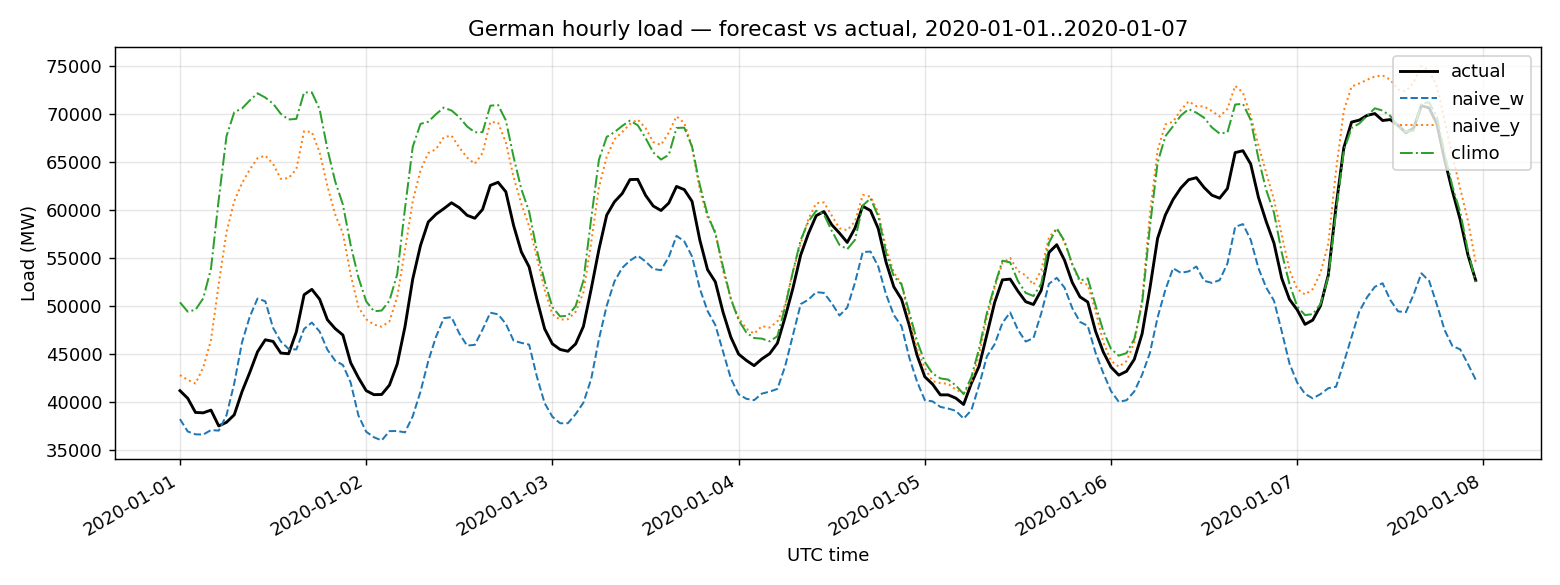
\includegraphics[height=0.62\textheight]{../runs/L1/forecast.png}
  \end{center}
  \begin{center}\small\color{gray!40!black}
    Three baselines compared; L1 picked the best of the three: \textbf{seasonal-naive (lag-364d), MAPE 10.76\%}.\\
    No transcript. No validation set. No prediction intervals.
  \end{center}
\end{frame}

% ===== Slide 9 — L2 prompt + AGENTS.md =====
\begin{frame}{L2 --- the average user}
  \begin{columns}[t,onlytextwidth]
    \begin{column}{0.48\textwidth}
      {\small\textbf{The prompt (46 words)}}\par\vspace{4pt}
      \codeblock{Build me a Python script that\\
forecasts German hourly electricity\\
load for the first week of January\\
2020 (the 168 hours from\\
2020-01-01 to 2020-01-07).\\
Train on the historical data,\\
produce the forecast, plot it\\
against the actual values, and\\
tell me how accurate it was.}
    \end{column}
    \begin{column}{0.48\textwidth}
      {\small\textbf{AGENTS.md (7 lines)}}\par\vspace{4pt}
      \codeblock{\# Notes for the AI\\[2pt]
Python project. The file\\
opsd\_de\_load.csv has hourly\\
German load (MW) from OPSD.\\[2pt]
Use pandas. Plot with matplotlib.}
    \end{column}
  \end{columns}
\end{frame}

% ===== Slide 10 — L2 output =====
\begin{frame}{L2 --- output}
  \begin{center}
    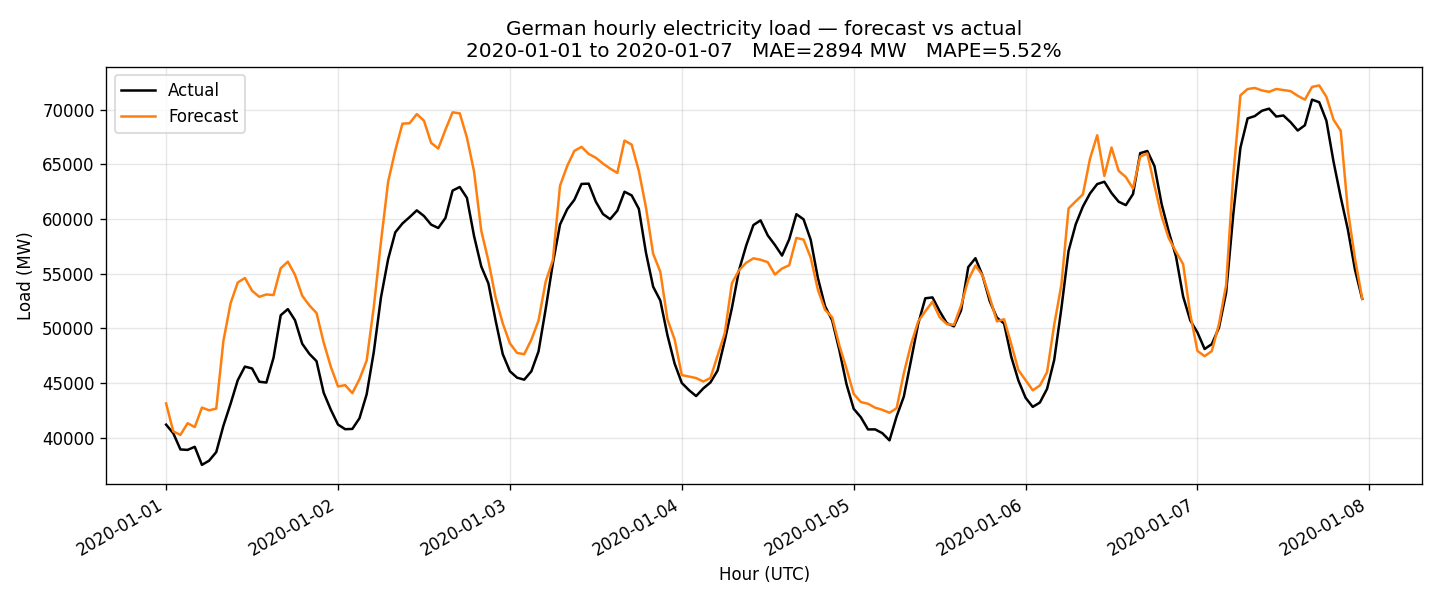
\includegraphics[height=0.62\textheight]{../runs/L2/forecast.png}
  \end{center}
  \begin{center}\small\color{gray!40!black}
    \textbf{GradientBoostingRegressor} with engineered features (hour, DOW, lag-168h, lag-8760h).\\
    \textbf{MAPE 5.52\%.} Still no transcript, no held-out validation, no intervals.
  \end{center}
\end{frame}

% ===== Slide 11 — L3 prompt + AGENTS.md =====
\begin{frame}{L3 --- the pro's prompt structure}
  \begin{columns}[t,onlytextwidth]
    \begin{column}{0.55\textwidth}
      \small\textbf{Prompt: 1{,}673 words}\par\vspace{4pt}
      \patternbox{taskblue}{TASK}{Forecast 168 hours. Six-model bake-off. Report MAPE / RMSE / MAE.}
      \patternbox{bggreen}{BACKGROUND}{Data \textperiodcentered{} Models \textperiodcentered{} Allowed inputs \textperiodcentered{} Splits \textperiodcentered{} Metrics \textperiodcentered{} Figures \textperiodcentered{} Outputs}
      \patternbox{dontred}{DO NOT}{Use the test window for fitting. Pull external data. Skip refit-on-train+val. Drop missing hours silently.}
    \end{column}
    \begin{column}{0.42\textwidth}
      \small\textbf{AGENTS.md: 113-line workspace file}\par\vspace{4pt}
      \begin{itemize}\small
        \item Allowed / Forbidden inputs
        \item \texttt{code/}, \texttt{figures/}, \texttt{metrics.json} output layout
        \item \texttt{metrics.json} JSON schema
        \item \texttt{Do NOT} block
        \item Style: plain language, type hints, no emoji
      \end{itemize}
    \end{column}
  \end{columns}
\end{frame}

% ===== Slide 12 — L3 winner with intervals =====
\begin{frame}{L3 --- the winner, with calibrated intervals}
  \begin{center}
    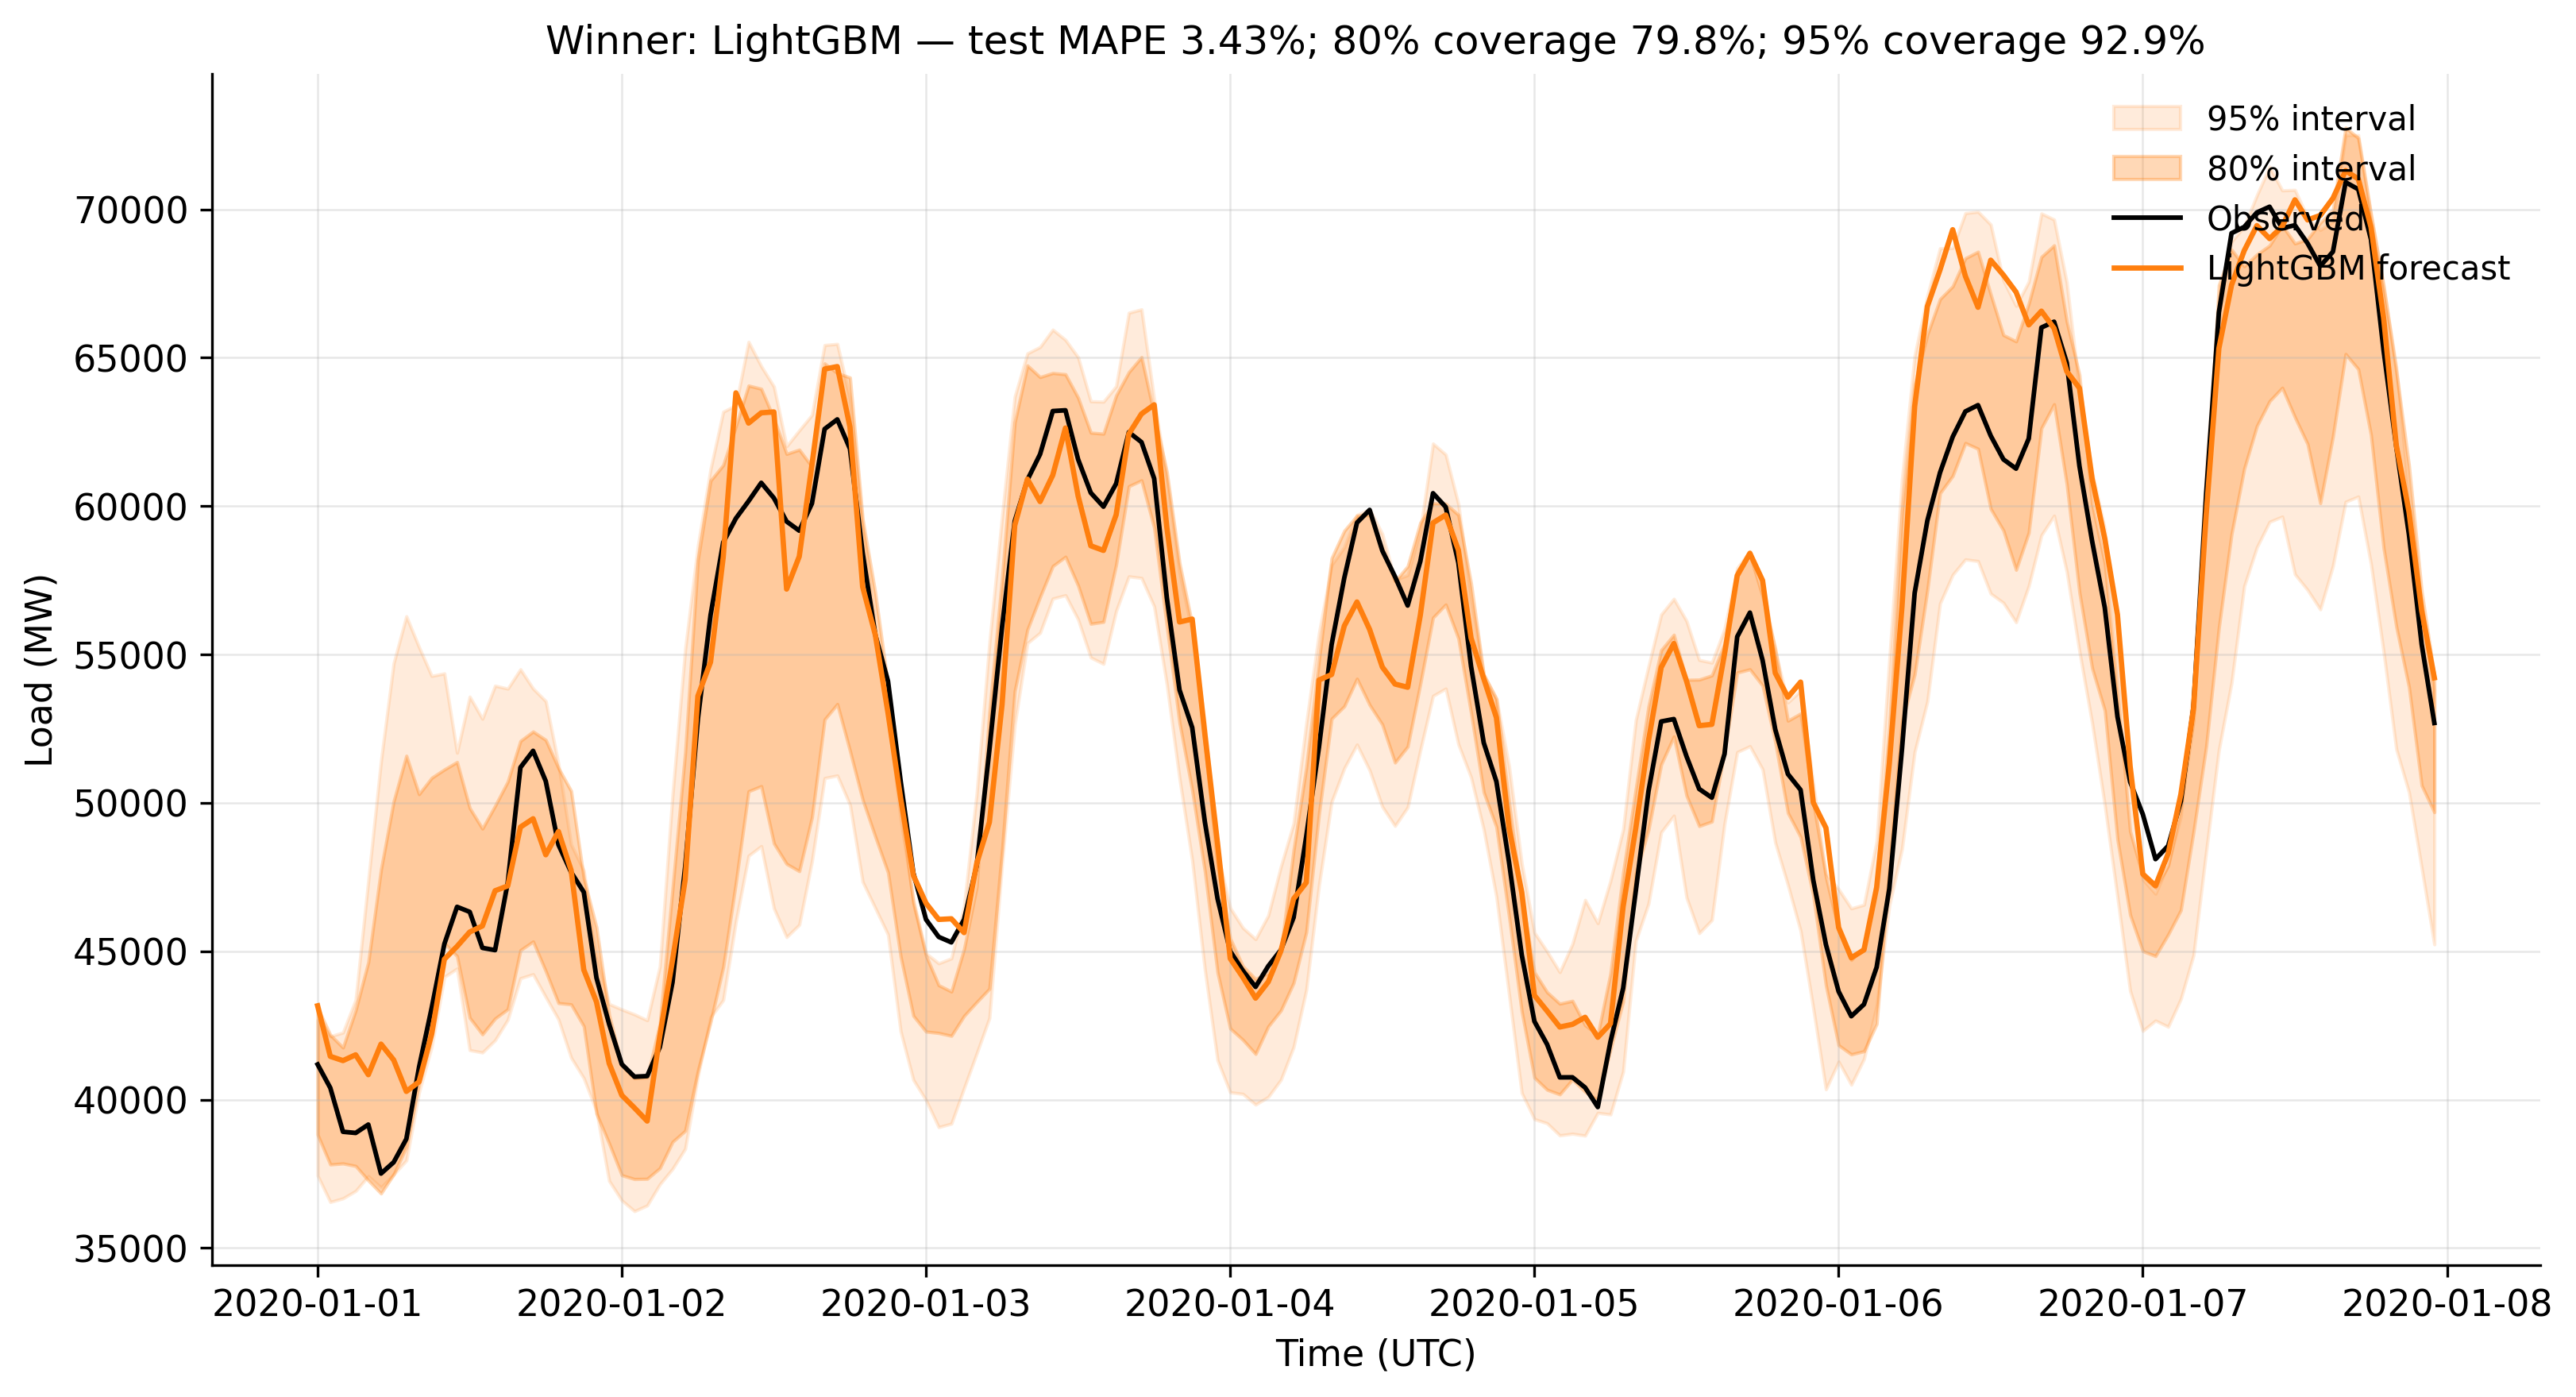
\includegraphics[height=0.66\textheight]{../runs/L3/figures/05_winner_with_intervals.png}
  \end{center}
  \begin{center}\small\color{gray!40!black}
    \textbf{LightGBM} on engineered features. \textbf{Test MAPE 3.43\%.}\\
    80\% PI covered 79.8\% of points \textperiodcentered{} 95\% PI covered 92.9\% --- essentially nominal.
  \end{center}
\end{frame}

% ===== Slide 13 — The bake-off =====
\begin{frame}{The bake-off --- six models}
  \begin{center}
    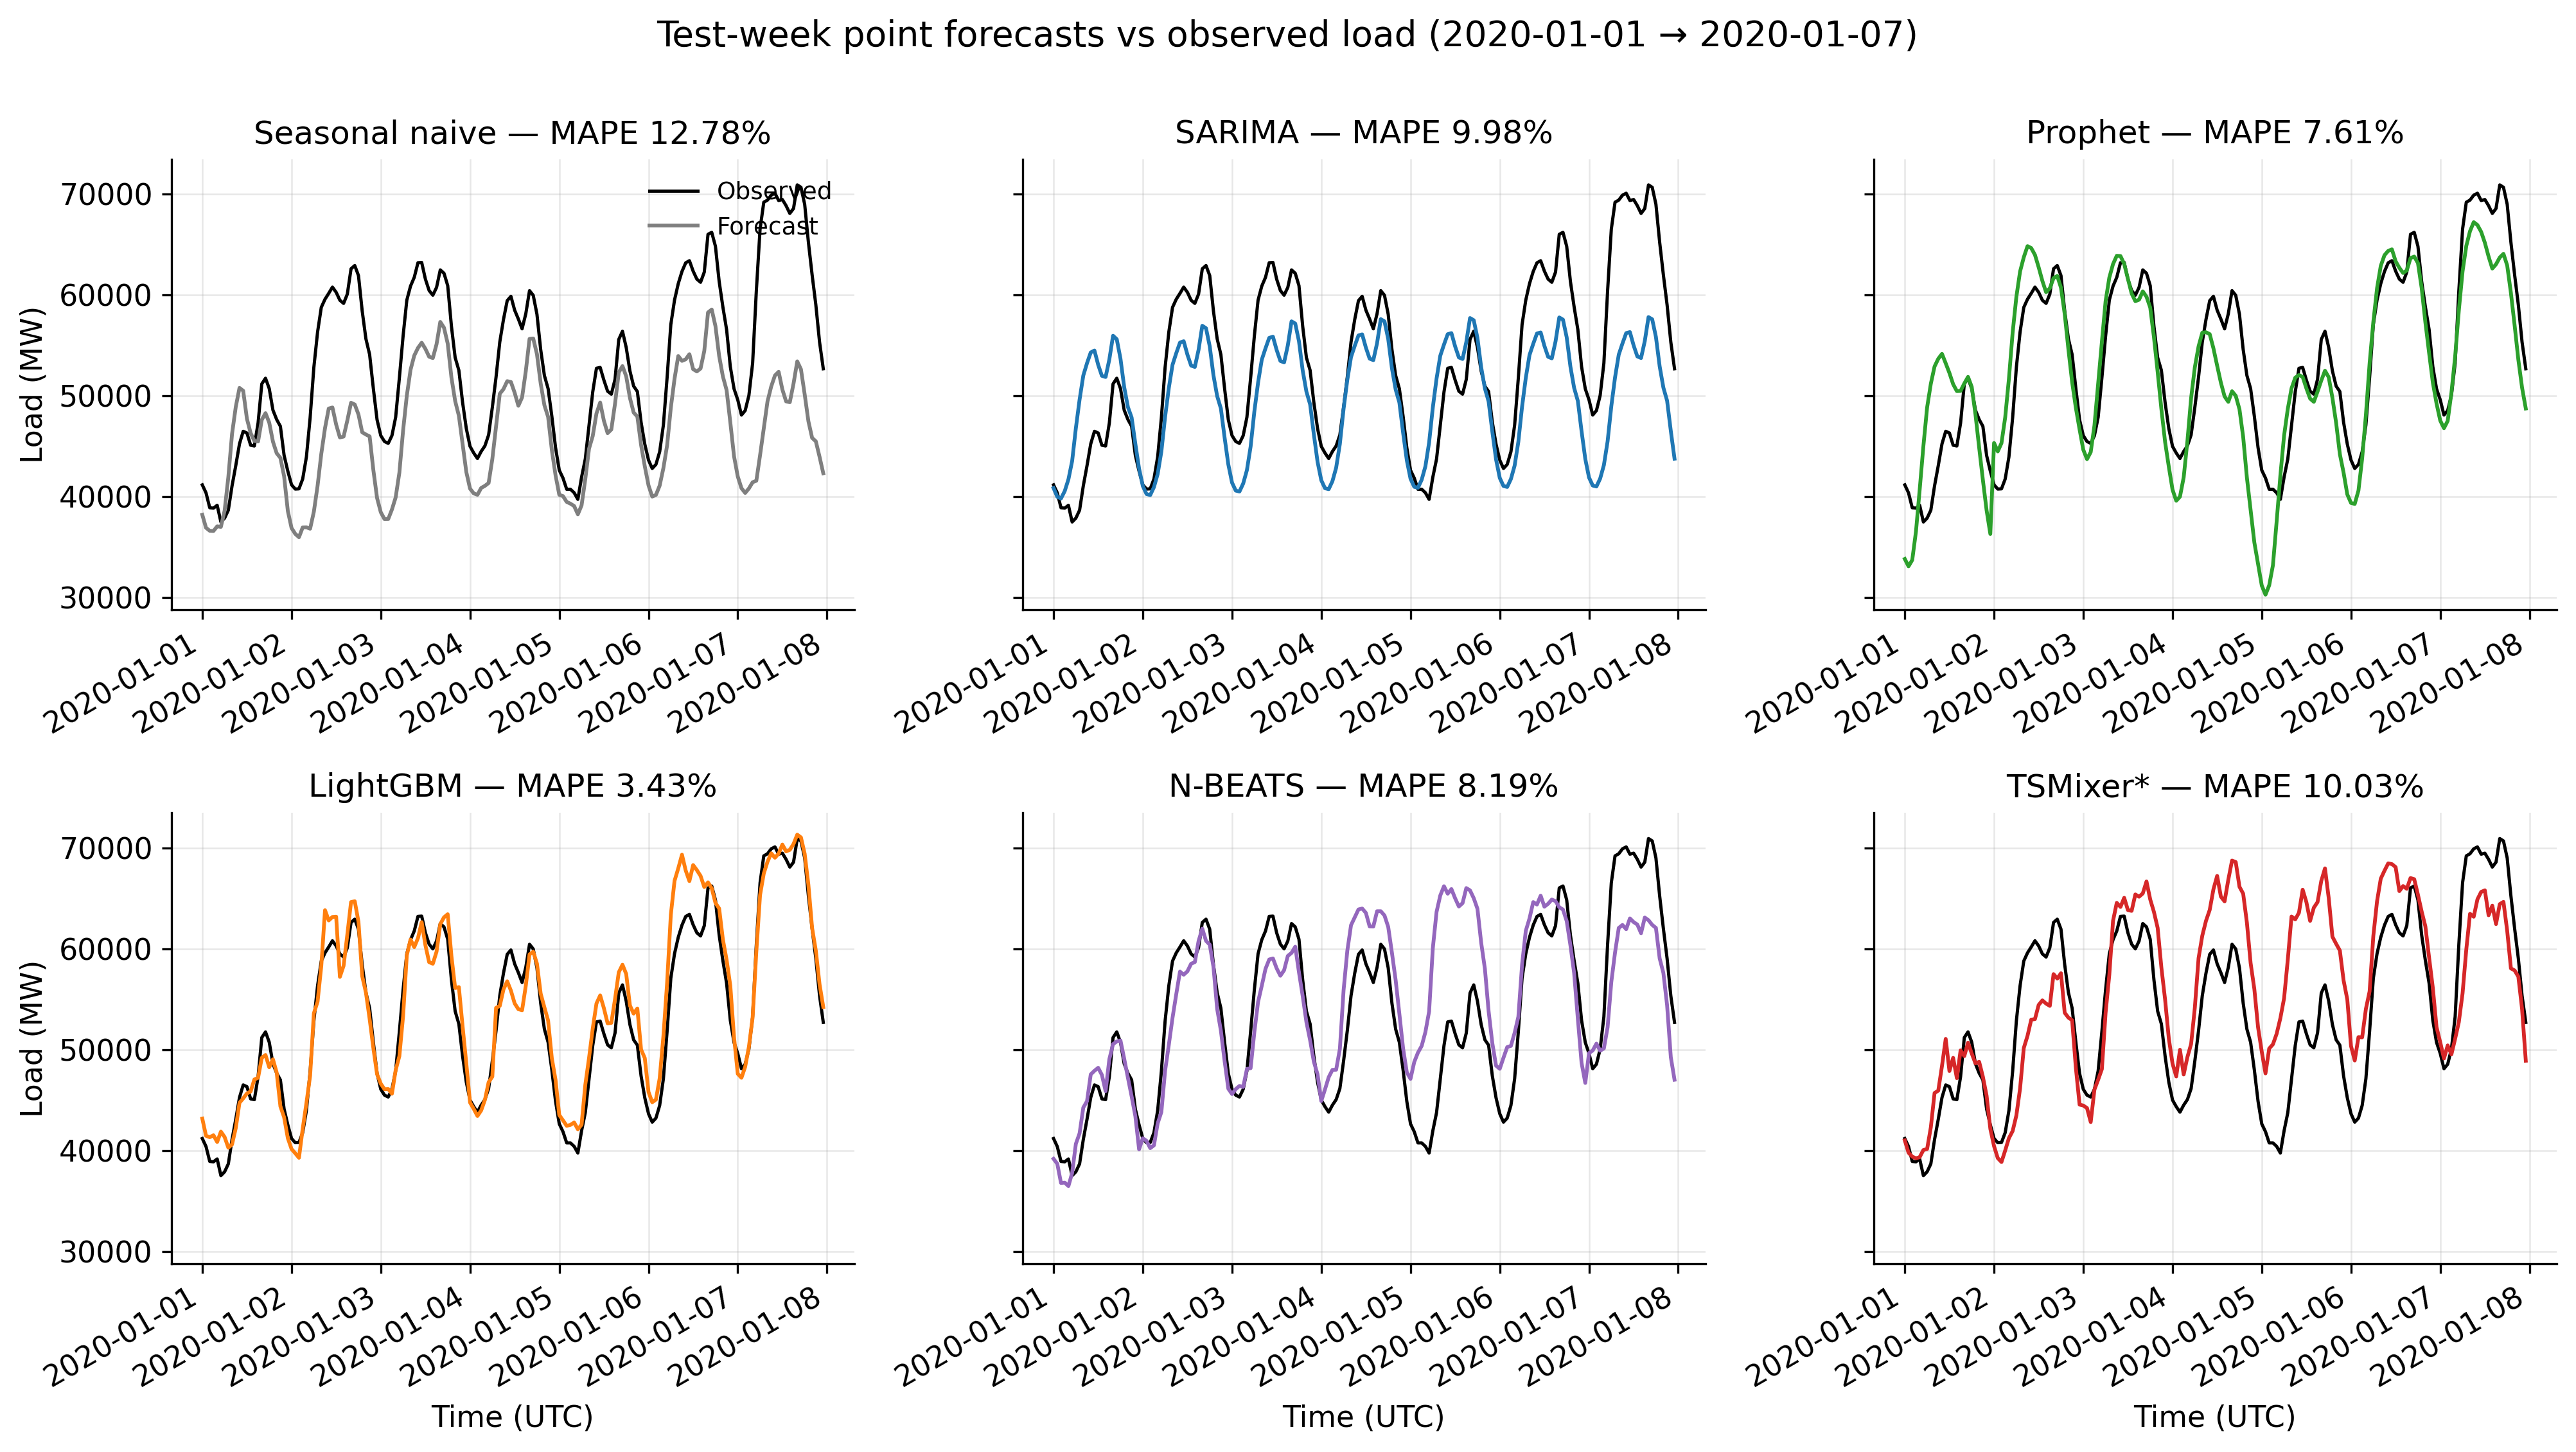
\includegraphics[height=0.72\textheight]{../runs/L3/figures/02_forecast_comparison.png}
  \end{center}
  \begin{center}\footnotesize\color{gray!40!black}
    Same train / validate / test splits. Same scoring window. One winner.
  \end{center}
\end{frame}

% ===== Slide 14 — Scoreboard =====
\begin{frame}{The scoreboard}
  \begin{center}
    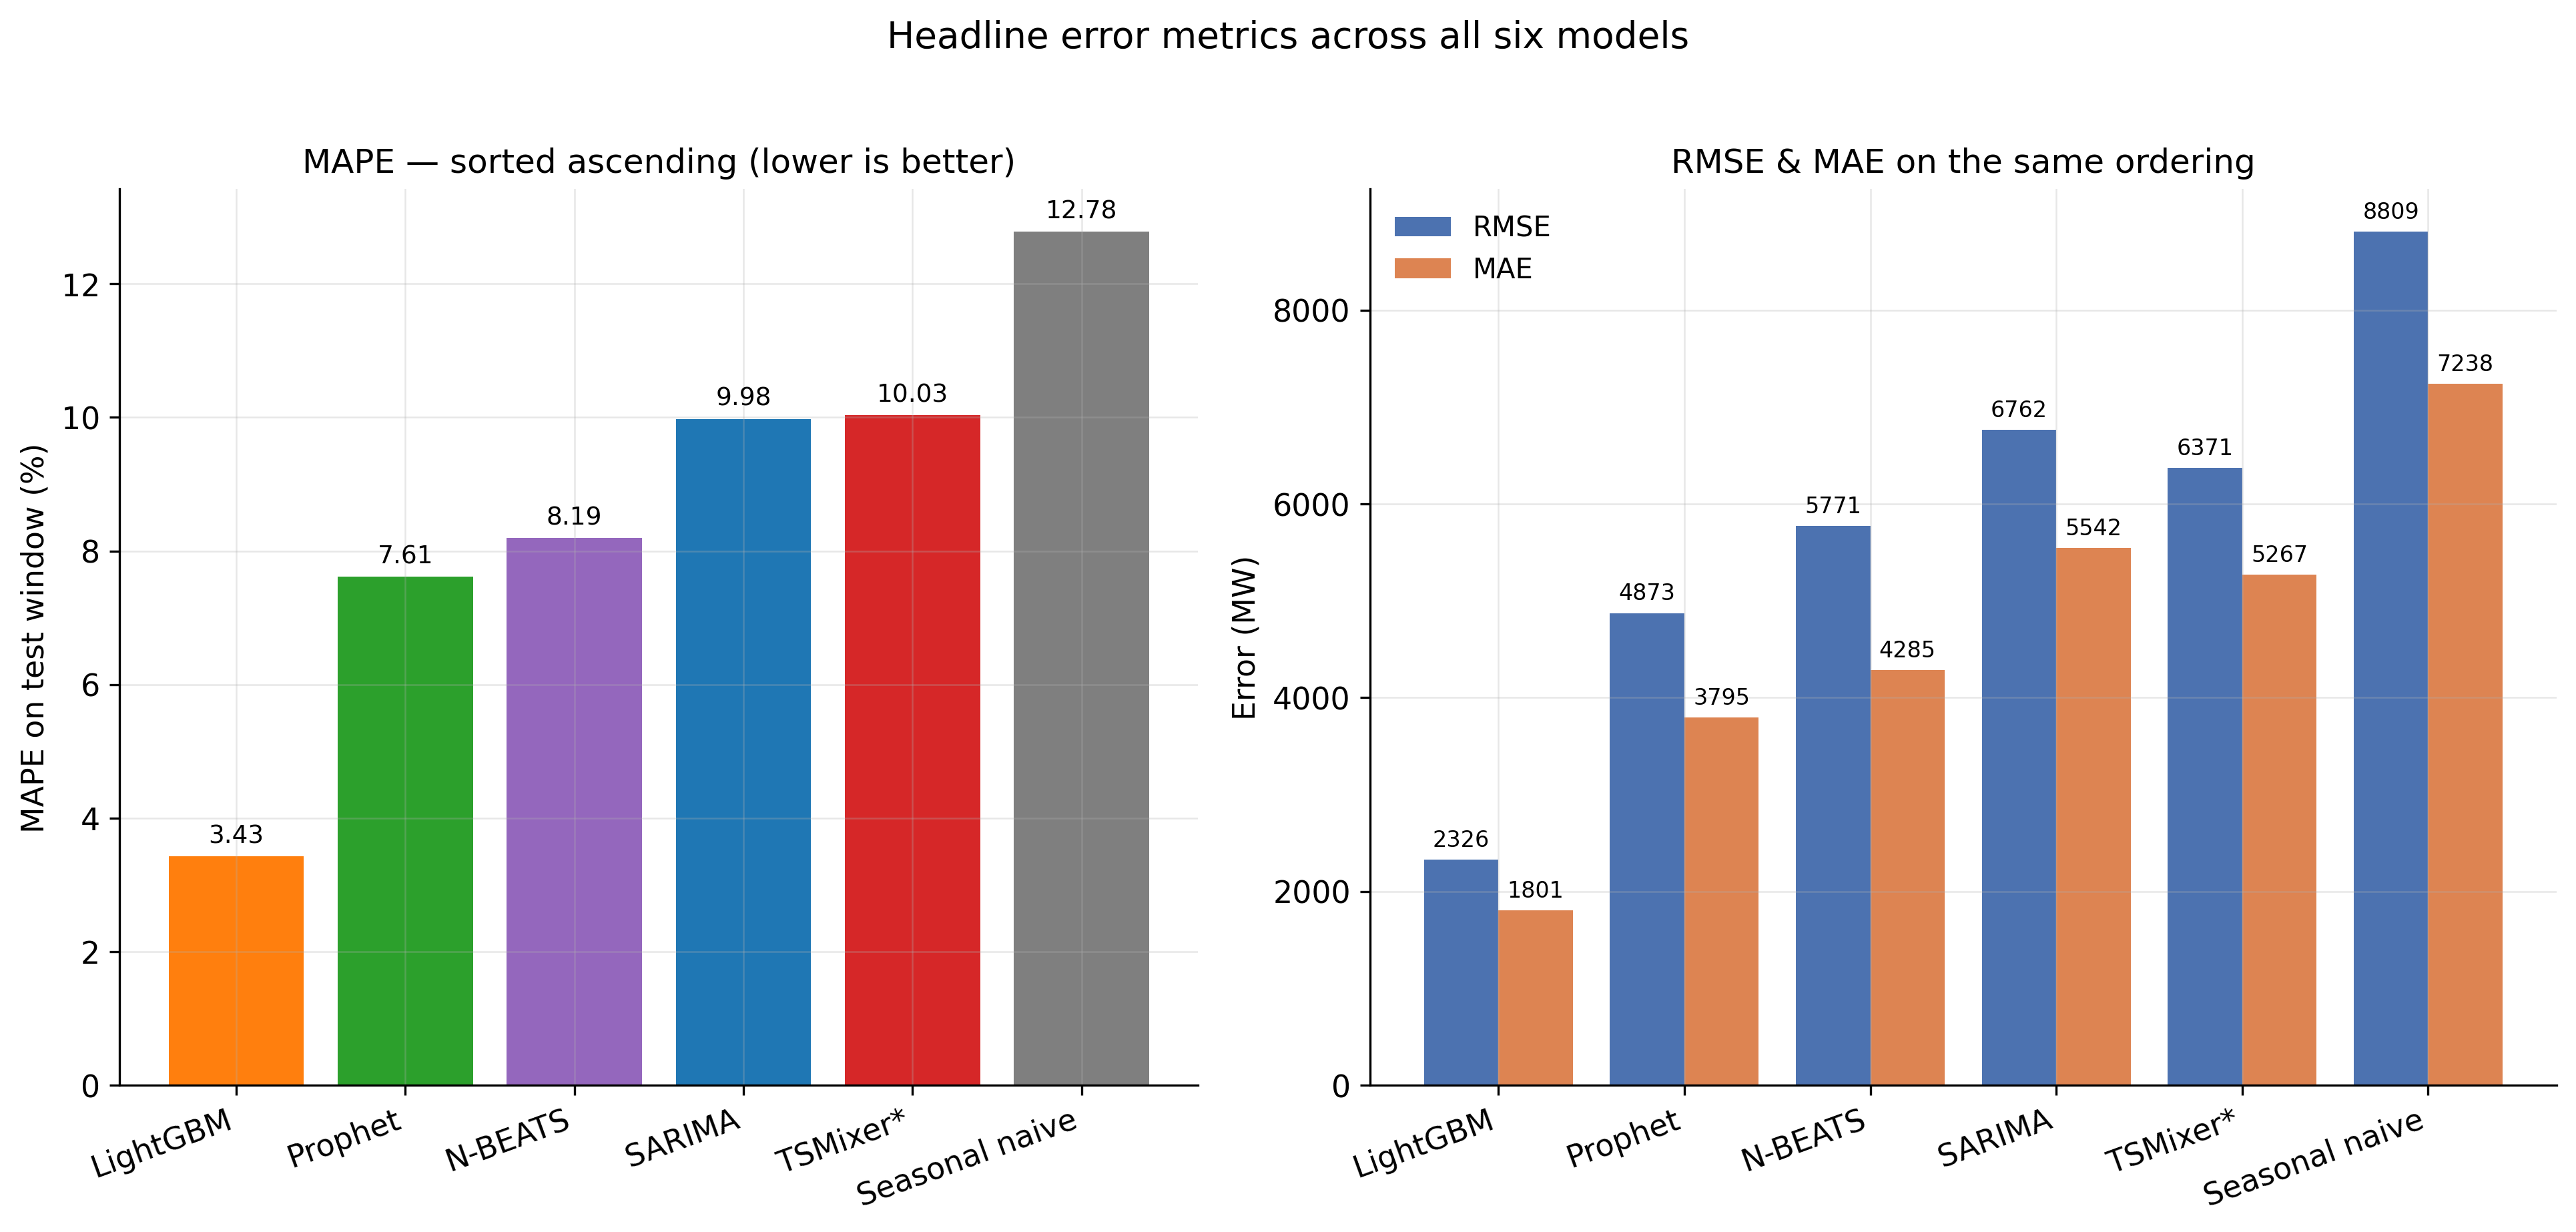
\includegraphics[height=0.68\textheight]{../runs/L3/figures/03_metric_comparison.png}
  \end{center}
  \begin{center}\small\color{gray!40!black}
    LightGBM wins MAPE, RMSE, and MAE simultaneously --- and is faster than three of the other five.
  \end{center}
\end{frame}

% ===== Slide 15 — Per-day diagnostic =====
\begin{frame}{Where each model fails --- per-day MAPE}
  \begin{center}
    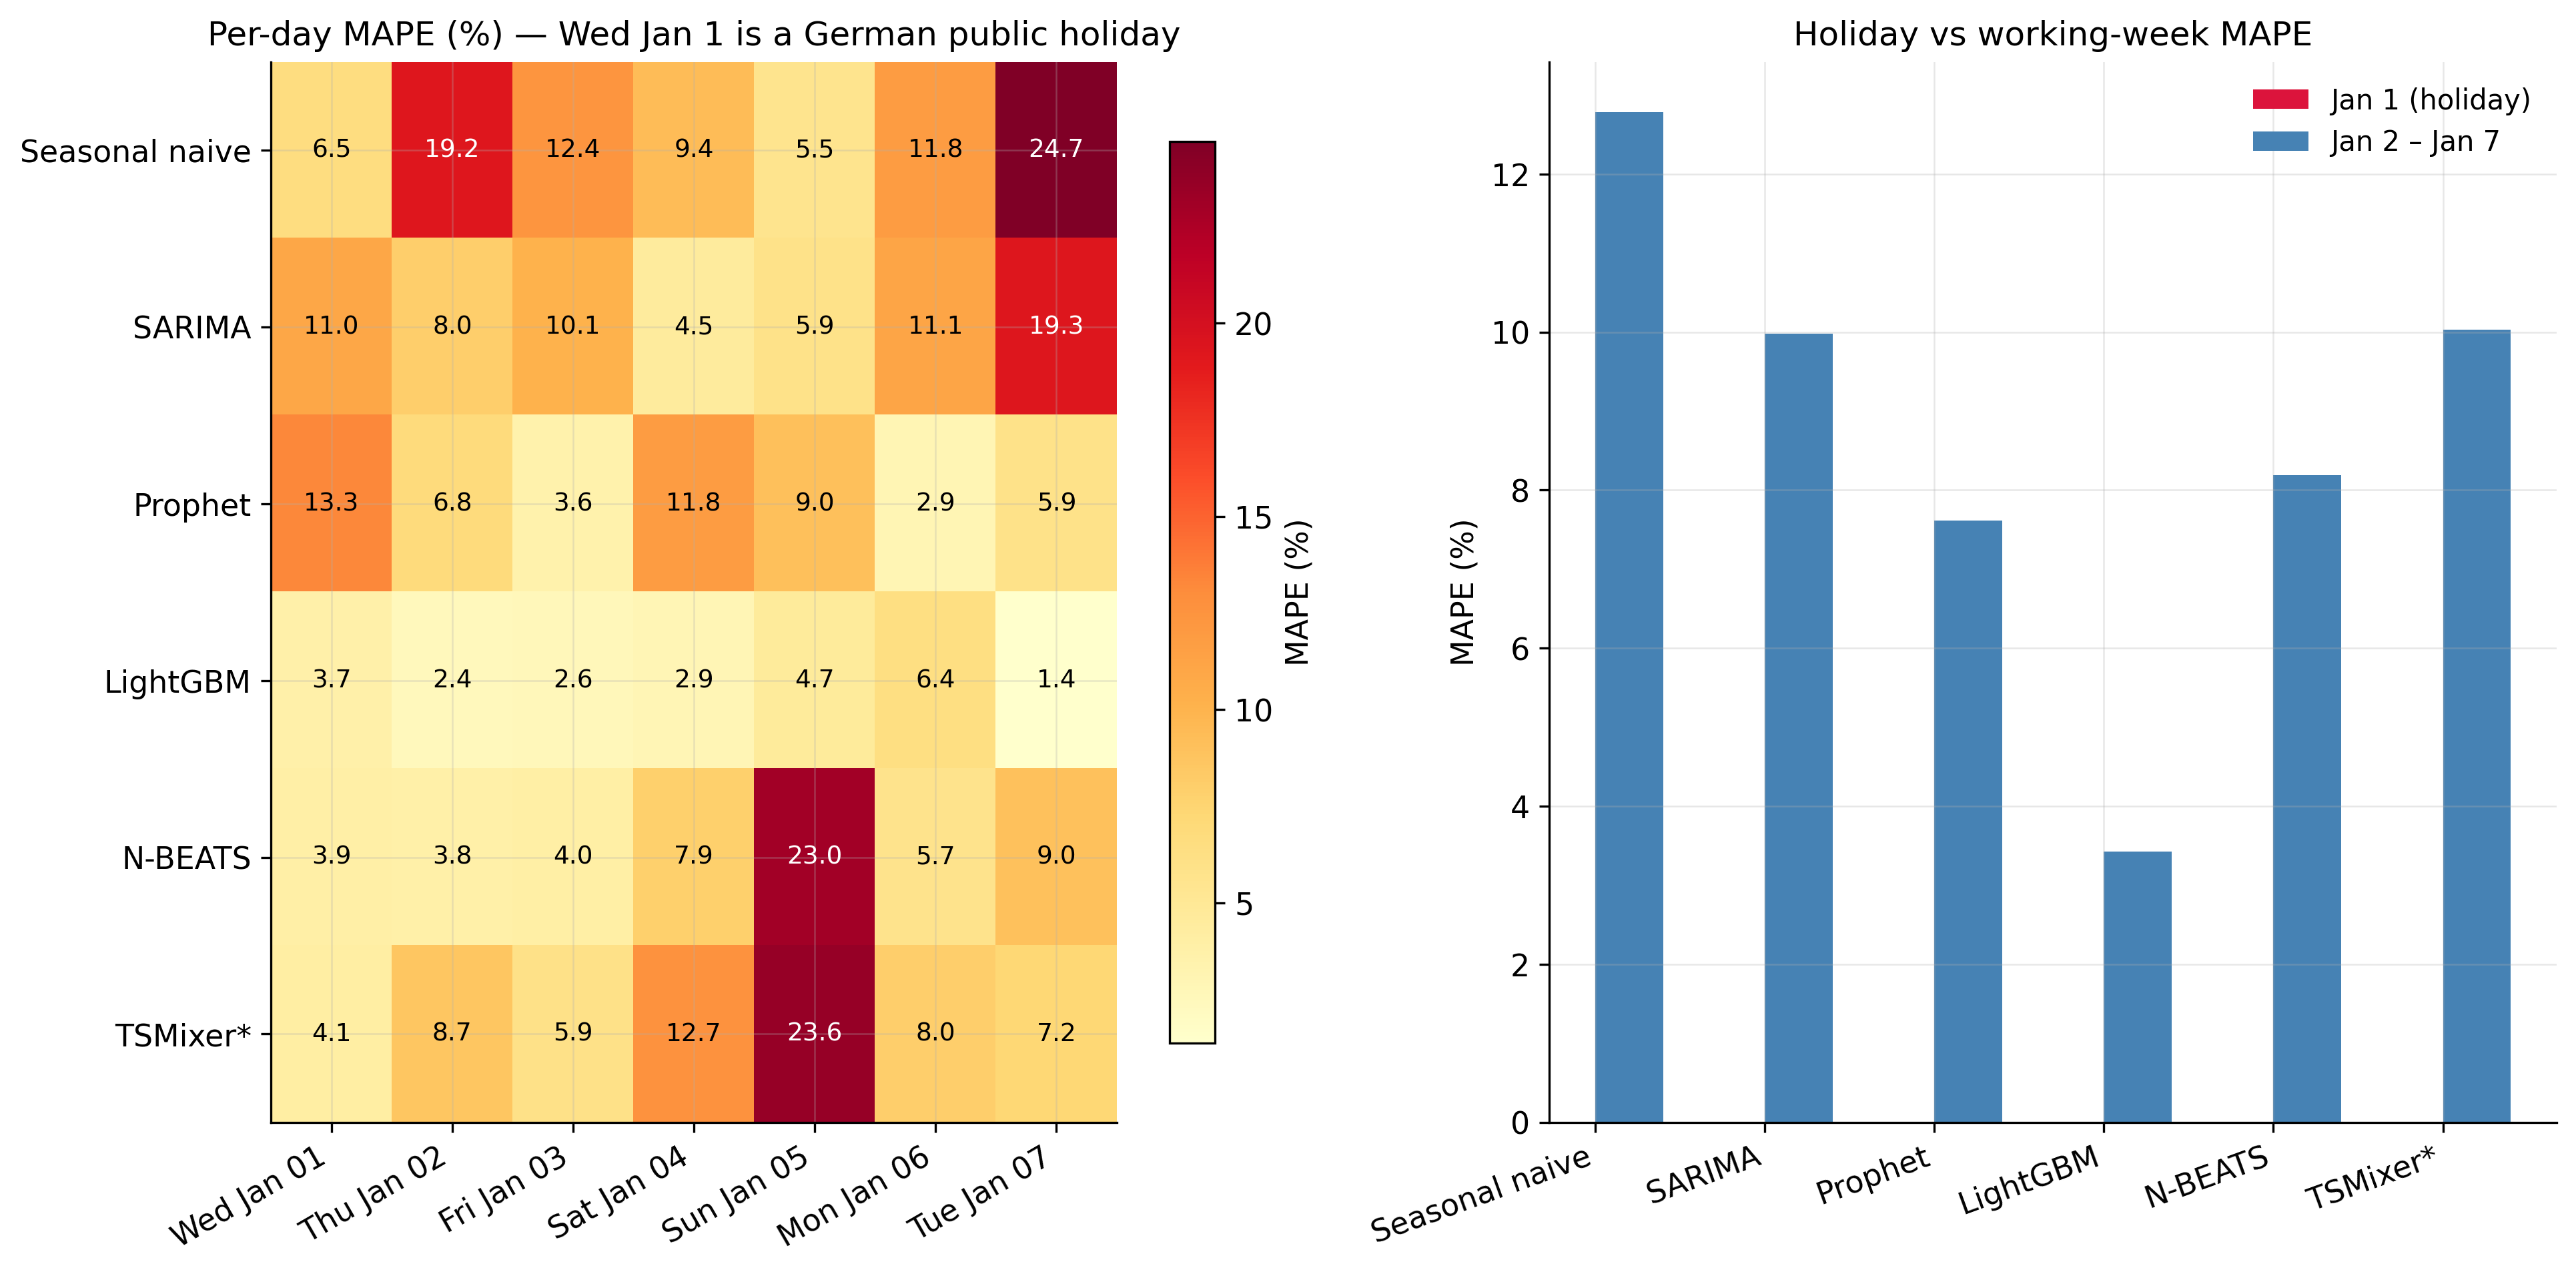
\includegraphics[height=0.68\textheight]{../runs/L3/figures/04_per_day_mape.png}
  \end{center}
  \begin{center}\small\color{gray!40!black}
    New Year's Day is the hardest day of the week. Only LightGBM stays uniformly low.
  \end{center}
\end{frame}

% ===== Slide 16 — Prompt length figure =====
\begin{frame}{What changed (1/4) --- the prompt itself}
  \begin{center}
    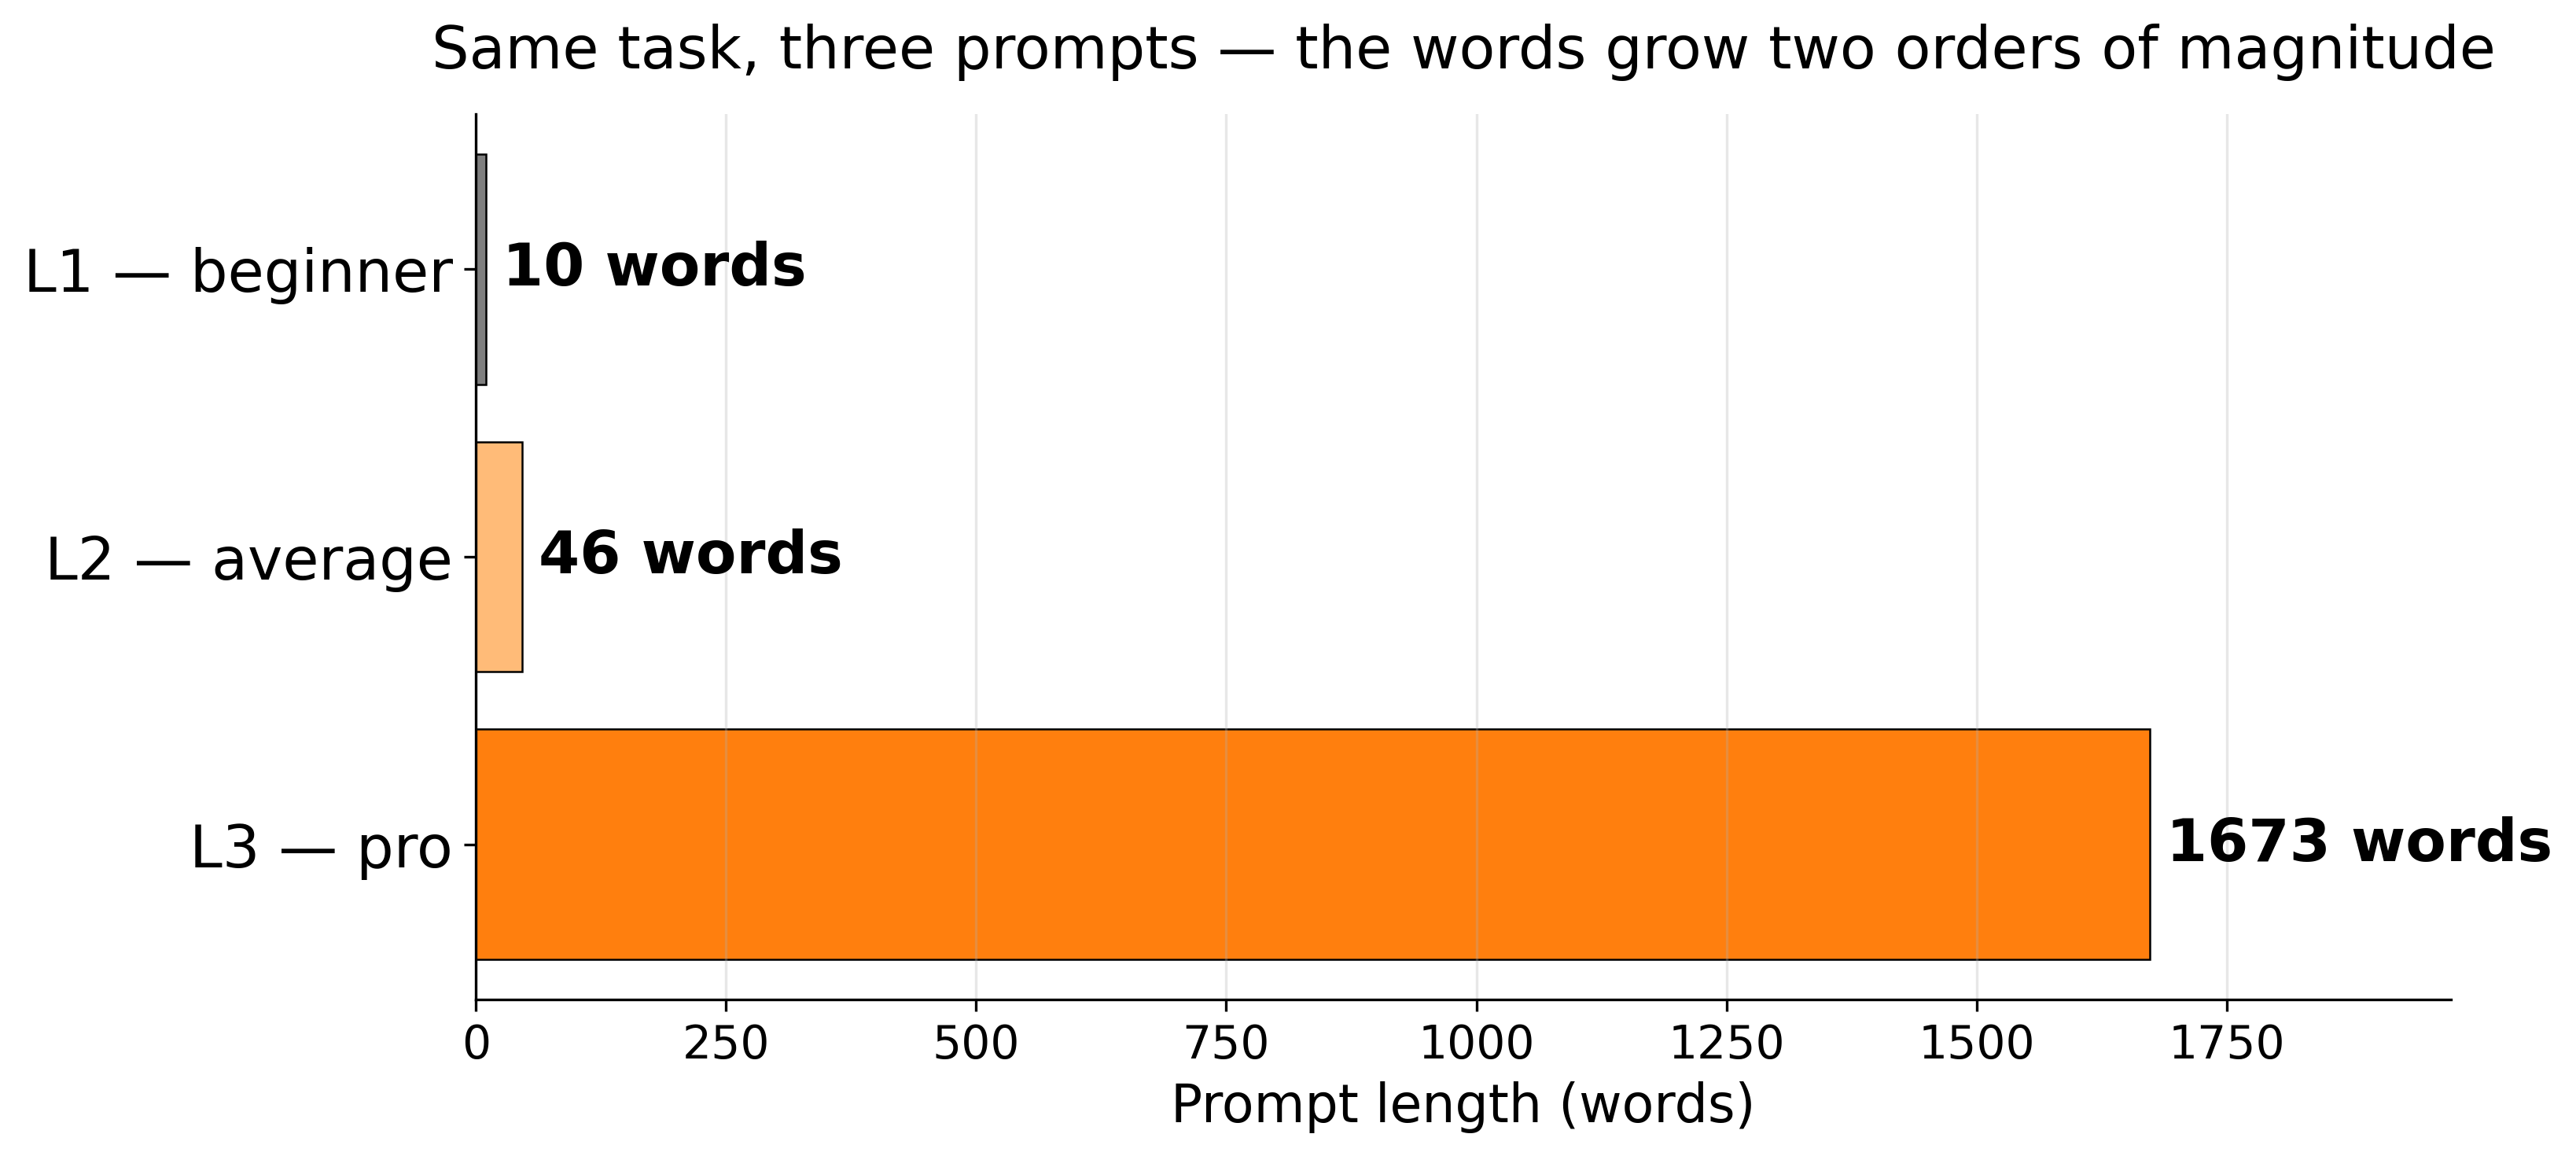
\includegraphics[width=0.85\textwidth]{assets/prompt_lengths.png}
  \end{center}
  \begin{center}\small\color{gray!40!black}
    \textbf{Video tip 2 --- be specific.} L3 isn't longer because the user is rambling;
    it's longer because every dimension that matters is named.
  \end{center}
\end{frame}

% ===== Slide 17 — AGENTS.md contrast =====
\begin{frame}{What changed (2/4) --- the project setup}
  \begin{columns}[t,onlytextwidth]
    \begin{column}{0.32\textwidth}
      \personacard{l1grey}{L1 --- AGENTS.md}{}{(none)}
    \end{column}
    \begin{column}{0.32\textwidth}
      \personacard{l2dark}{L2 --- AGENTS.md (7 lines)}{}{Data file location \textperiodcentered{} pandas + matplotlib}
    \end{column}
    \begin{column}{0.32\textwidth}
      \personacard{l3orange}{L3 --- AGENTS.md (113 lines)}{}{Allowed / Forbidden inputs \textperiodcentered{} Output schema \textperiodcentered{} \texttt{metrics.json} contract \textperiodcentered{} Do-NOT block \textperiodcentered{} Style}
    \end{column}
  \end{columns}
  \vspace{8pt}
  \begin{center}\small\color{gray!40!black}
    \textbf{Video tip 5 --- tell the AI to remember.} AGENTS.md is read at the start of every
    session. It's the single biggest leverage point most people miss.
  \end{center}
\end{frame}

% ===== Slide 18 — TASK/BG/DO-NOT =====
\begin{frame}{What changed (3/4) --- the DO NOT pattern}
  \patternbox{taskblue}{TASK}{What to do, precisely. The objective, the metric, the output shape.}
  \patternbox{bggreen}{BACKGROUND}{Data, files, constraints, references the model needs to do the task well.}
  \patternbox{dontred}{DO NOT}{What to avoid. The cheapest, highest-leverage section of any prompt.}
  \vspace{4pt}
  \begin{center}\small\color{gray!40!black}
    \textbf{Video tip 4 --- the DO NOT pattern.} Our L3 prompt has nine specific don'ts.
    The one that mattered most: \emph{do not use the test window for fitting.}
  \end{center}
\end{frame}

% ===== Slide 19 — Validation =====
\begin{frame}{What changed (4/4) --- ask for verification}
  \begin{columns}[t,onlytextwidth]
    \begin{column}{0.48\textwidth}
      \textbf{\textcolor{l1grey}{L1}}\par\vspace{4pt}
      \small No held-out validation set. No calibrated intervals. Reports test-set MAPE only.\par\vspace{6pt}
      The forecasts use only pre-test lags and climatology --- there is no data leakage. Just no methodological discipline above what the agent thought to add unprompted.
    \end{column}
    \begin{column}{0.48\textwidth}
      \textbf{\textcolor{l3orange}{L3}}\par\vspace{4pt}
      \small Train (2015 $\to$ 2019-09-30) $\to$ validate (2019-10--12) $\to$ refit on train+val $\to$ forecast 2020-01-01..07.\par\vspace{6pt}
      80\% PI covered \textbf{79.8\%} \textperiodcentered{} 95\% PI covered \textbf{92.9\%}. Essentially nominal.
    \end{column}
  \end{columns}
  \vspace{6pt}
  \begin{center}\small\color{gray!40!black}
    \textbf{Video tip 7 --- always verify.} Calibration doesn't happen by accident.
    It happens because you asked.
  \end{center}
\end{frame}

% ===== Slide 20 — So what =====
\begin{frame}{So what --- four habits}
  \vspace{8pt}
  \begin{enumerate}\large
    \item \textbf{Specify what success looks like} --- not just what to build.
    \item \textbf{Use a DO NOT section} --- including the obvious-but-easy-to-miss ones.
    \item \textbf{Put standing context in \texttt{AGENTS.md}} --- once, not every session.
    \item \textbf{Make the AI verify itself} --- backtest, intervals, written discussion.
  \end{enumerate}
  \vspace{10pt}
  \begin{center}\small\color{gray!40!black}
    Same four habits whether you're forecasting load, drafting a paper, or searching the literature.
  \end{center}
\end{frame}

% ===== Slide 21 — Closer =====
{\setbeamertemplate{footline}{}
\begin{frame}[plain]
  \vfill
  \begin{center}
    {\fontsize{52pt}{56pt}\selectfont\bfseries\textcolor{l3orange}{Your goal is leverage.}}
  \end{center}
  \vspace{20pt}
  \begin{center}
    {\Large\textcolor{gray!40!black}{AI scales execution. Humans bring the ideas and the judgement.}}
  \end{center}
  \vfill
  \begin{center}\small\itshape\textcolor{gray}{after The Coding Sloth, 2025 \quad\textperiodcentered\quad code \& data: github.com/DermotOBrien-EC/LLM\_coding\_example\_jrc\_andres}\end{center}
\end{frame}}

\end{document}
